\chapter{The Full EO Pipeline: Tiling, Inference, GeoTIFF}
\label{ch:pipeline}

\chapmeta{Advanced}{$\sim$6\,h (2\,h + 4\,h)}{Sentinel-2 scenes (synthetic + real)}

\begin{objbox}
\begin{itemize}[leftmargin=1.2em,nosep]
  \item Assemble a complete pipeline: raw scene $\to$ tiles $\to$ inference $\to$ map.
  \item Implement memory-safe sliding-window inference over a full Sentinel-2 tile.
  \item Blend overlapping predictions with Gaussian weighting to remove seams.
  \item Export a georeferenced GeoTIFF with correct CRS and transform.
  \item Compute per-class area statistics from a prediction map.
\end{itemize}
\end{objbox}

This chapter closes the loop: a trained segmentation model becomes a deployable
system that turns a $\sim$$10980\times10980$ Sentinel-2 scene into a
georeferenced land-cover map. No single GPU can hold such a scene, so inference
must be tiled, and the tiles' predictions stitched back into one seamless raster.

\section{Pipeline overview}

The end-to-end flow chains the components built in earlier chapters
(Figure~\ref{fig:pipe}): load and preprocess the scene
(Chapter~\ref{ch:preproc}), tile it with overlap, run the model on each tile
(Chapters~\ref{ch:seg}--\ref{ch:advseg}), blend predictions, reconstruct the
full map, and write a GeoTIFF.

\begin{figure}[h]
\centering
\begin{tikzpicture}[font=\scriptsize,>=Latex,node distance=5mm]
  \tikzstyle{b}=[draw,rounded corners,minimum height=8mm,minimum width=20mm,align=center]
  \node[b,fill=eoblue!10] (a){Raw scene\\(GeoTIFF)};
  \node[b,fill=eoblue!10,right=of a] (p){Preprocess\\norm + indices};
  \node[b,fill=eoearth!12,right=of p] (t){Tile\\(overlap)};
  \node[b,fill=eogreen!12,right=of t] (m){Model\\per tile};
  \node[b,fill=eogreen!12,below=7mm of m] (bl){Gaussian\\blend};
  \node[b,fill=eoearth!12,left=of bl] (rc){Reconstruct\\full map};
  \node[b,fill=eored!12,left=of rc] (g){Export\\GeoTIFF};
  \draw[->](a)--(p);\draw[->](p)--(t);\draw[->](t)--(m);\draw[->](m)--(bl);
  \draw[->](bl)--(rc);\draw[->](rc)--(g);
\end{tikzpicture}
\caption{The full inference pipeline. Every stage corresponds to a tool built in
an earlier chapter; only the orchestration is new.}
\label{fig:pipe}
\end{figure}

\section{Sliding-window inference}

We slide a $T\times T$ window with stride $s<T$ (overlap $T-s$) across the
scene. For each window we run the model to obtain class \emph{probabilities}
(not hard labels --- we need to average), and accumulate them into a full-scene
buffer $P\in\R^{K\times H\times W}$ together with a weight buffer $A$. The final
per-pixel prediction is $\arg\max_k P[k]/A$.
\begin{lstlisting}
import numpy as np, torch
def sliding_window(model, scene, T=512, s=384, K=7, device="cuda"):
    C, H, W = scene.shape
    P = np.zeros((K, H, W), np.float32); A = np.zeros((H, W), np.float32)
    wmap = gaussian_weight(T)                      # (T, T), peaks at centre
    model.eval()
    with torch.no_grad():
        for y in range(0, H - T + 1, s):
            for x in range(0, W - T + 1, s):
                tile = torch.from_numpy(scene[:, y:y+T, x:x+T])[None].to(device)
                prob = model(tile).softmax(1)[0].cpu().numpy()   # (K, T, T)
                P[:, y:y+T, x:x+T] += prob * wmap
                A[y:y+T, x:x+T]    += wmap
    return (P / np.maximum(A, 1e-6)).argmax(0)     # (H, W) labels
\end{lstlisting}
Edge handling (padding the last partial tile) and batching multiple tiles
together for throughput are the practical refinements.

\section{Why Gaussian blending}

If overlapping tiles are averaged with equal weight, predictions near a tile's
border --- where the receptive field is truncated and context is missing --- are
unreliable and produce visible grid \emph{seams}. Weighting each tile by a 2D
Gaussian $w(u,v)\propto\exp\!\big(-\tfrac{(u-c)^2+(v-c)^2}{2\sigma^2}\big)$
centred on the tile (so centre pixels dominate, borders fade) makes the
contributions of adjacent tiles transition smoothly, eliminating seams. The
ablation ``equal weight vs Gaussian'' makes the artefact and its cure obvious.

\section{Georeferenced export}

A prediction is useless to a GIS analyst unless it carries its geolocation. We
write the label raster with the \emph{same} CRS and affine transform as the
input scene, so it overlays exactly in QGIS:
\begin{lstlisting}
import rasterio
with rasterio.open(src_path) as src:
    profile = src.profile
profile.update(count=1, dtype="uint8", nodata=0)
with rasterio.open("landcover.tif", "w", **profile) as dst:
    dst.write(pred.astype("uint8"), 1)
    dst.write_colormap(1, {i: hex_to_rgb(c) for i, c in enumerate(PALETTE)})
\end{lstlisting}
Embedding a colour map renders the classes correctly without manual styling.

\section{Area statistics}

Because each pixel covers a known ground area ($10\times10\,\mathrm{m}=100\,
\mathrm{m}^2$ for Sentinel-2 10\,m bands), counting pixels per class converts
directly to hectares:
\begin{equation}
\text{area}_k\,[\mathrm{ha}] = \frac{n_k \cdot A_\mathrm{px}}{10^4},
\qquad A_\mathrm{px}=|a\cdot e|\ \mathrm{m}^2,
\end{equation}
turning a colourful map into the quantitative output stakeholders actually want
(``X hectares of forest, Y of built-up''). Figure~\ref{fig:lc} shows a
representative scene and its predicted land-cover map.

\begin{figure}[h]
\centering
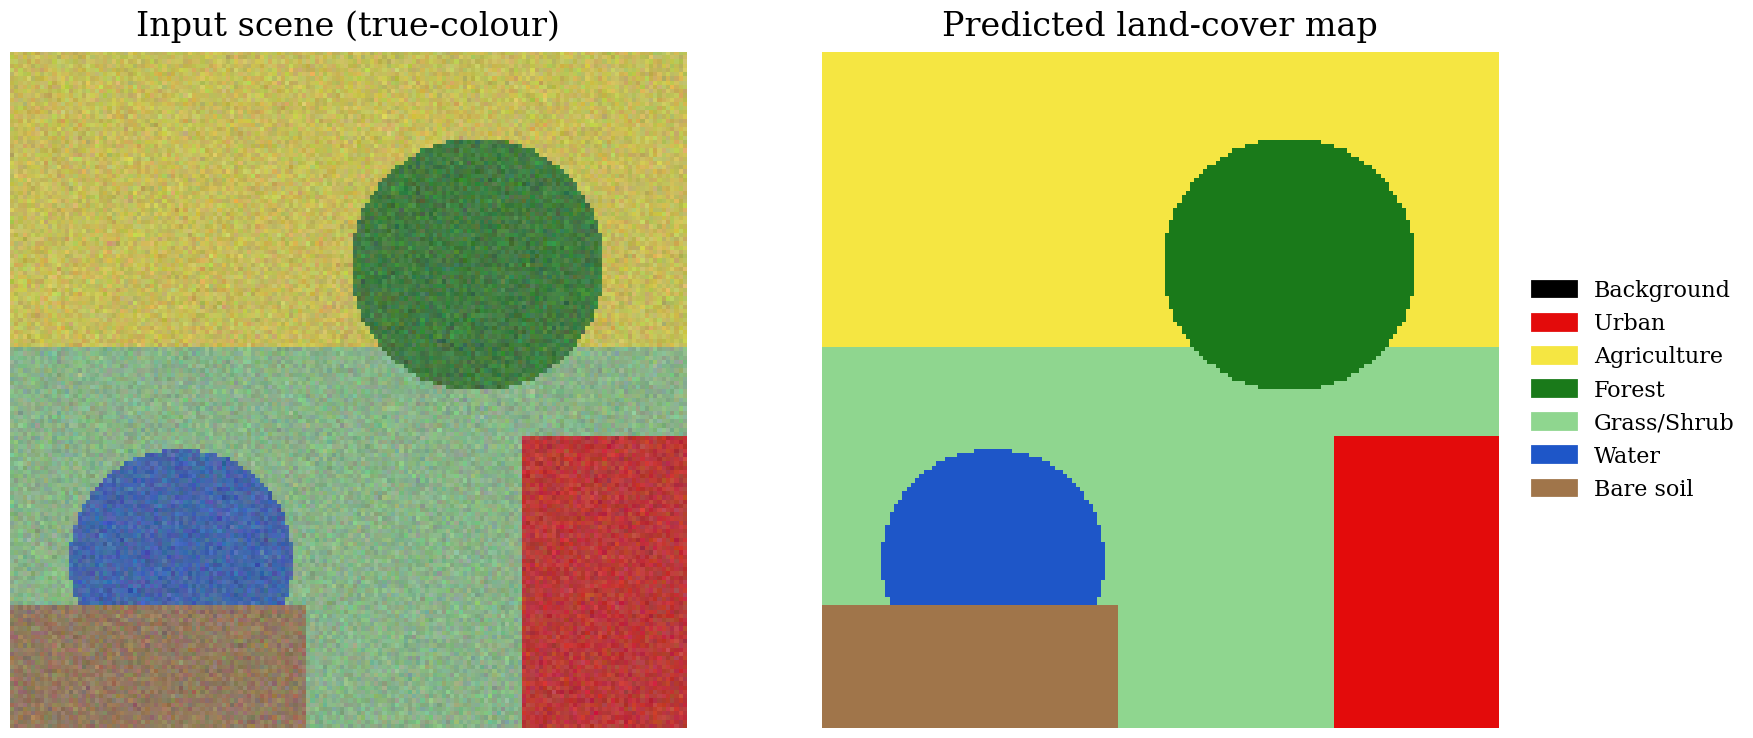
\includegraphics[width=0.95\linewidth]{figures/landcover.png}
\caption{Input scene (left) and reconstructed land-cover prediction (right) with
a class legend --- the deliverable of the full pipeline and of the capstone.}
\label{fig:lc}
\end{figure}

\begin{keybox}
\begin{itemize}[leftmargin=1.2em,nosep]
  \item Full-scene inference is tiled; accumulate \emph{probabilities}, then argmax.
  \item Overlap + Gaussian blending removes tile seams from truncated-context borders.
  \item Export with the source CRS/transform (and a colour map) for GIS-ready GeoTIFFs.
  \item Pixel area $\to$ hectares gives quantitative, decision-ready statistics.
  \item The pipeline is pure orchestration of tools from Chapters~\ref{ch:preproc}--\ref{ch:advseg}.
\end{itemize}
\end{keybox}

\begin{practbox}
Notebook: \nbpath{chapter\_11\_full\_eo\_pipeline/11\_practical\_end\_to\_end\_pipeline.ipynb}.
\begin{enumerate}[leftmargin=1.4em,nosep]
  \item Create (or load) a large multi-band scene with spatial structure.
  \item Implement \texttt{gaussian\_weight} and the sliding-window inference loop.
  \item Run inference with a trained (or demo) model; reconstruct the full map.
  \item Compare reconstructions \emph{with} and \emph{without} Gaussian blending.
  \item Export a georeferenced GeoTIFF with a colour map; compute per-class hectares.
\end{enumerate}
\end{practbox}

\begin{exbox}
\textbf{11.1 Overlap effect.} Sweep stride/overlap; quantify seam artefacts and
runtime trade-offs.\\[2pt]
\textbf{11.2 Batched tiles.} Batch multiple tiles per forward pass; measure the
throughput gain.\\[2pt]
\textbf{11.3 QGIS check.} Open your GeoTIFF in QGIS over an OSM basemap; verify
alignment and discuss any offset.\\[2pt]
\textbf{Mini-project.} Wrap the pipeline into \texttt{predict\_scene(model,
path) -> geotiff} with a CLI, then run it on a real downloaded Sentinel-2 tile.
\end{exbox}
